\documentclass{article}
\usepackage[spanish,es-lcroman,activeacute,es-tabla] {babel}
\usepackage[utf8]{inputenc}
\usepackage[pdftex, plainpages=false, hypertexnames=false, pdfpagelabels=true,
    hyperindex=true, linktocpage, pagebackref=true, pdfa=true]{hyperref}         % Vinculos
\usepackage{graphicx}
\usepackage[left=3cm,top=3cm,right=3cm,bottom=3cm]{geometry} %%Márgenes
\usepackage{subcaption}
\usepackage{caption}
\usepackage{amsmath}
\usepackage{color}
\usepackage{float}			
\usepackage{parskip}				
\usepackage{listingsutf8}			%Incluir códigos
\spanishplainpercent					%Habilitar % en códigos sin comentar
\usepackage{xcolor}						%Generar mezclas de colores
\usepackage{advdate}					%Avance de fechas

%Eliminar bordes rojos de los hipervinculos
\hypersetup{pdfborder=0 0 0}
%Empezar con pantalla a lo ancho
%\hypersetup{pdfstartview={XYZ null null 1.00}}

\definecolor{DarkGreen}{RGB}{0,128,0}

\lstset{
	keywordstyle=\color{blue}\bfseries,
    commentstyle=\color{DarkGreen},
	basicstyle=\ttfamily\small,
    numberstyle=\footnotesize,
    backgroundcolor=\color{gray!10},
    frame=single,
    tabsize=2,
    rulecolor=\color{black!30},
    %title=\lstname,
    escapeinside={\%*}{*)},
    breaklines=true,
    breakatwhitespace=true,
    framextopmargin=2pt,
    framexbottommargin=2pt,
    inputencoding=utf8,
    extendedchars=true,
    literate={á}{{\'a}}1 {í}{{\'a}}1 {é}{{\'e}}1 {ó}{{\'o}}1 {ú}{{\'u}}1 {ñ}{{\~n}}1 {"}{{''}}1,
}


\setlength{\parskip}{3.1mm plus2mm minus2mm}

%\title{Resumen Artículo Paralelización de Motion JPEG 2000 con CUDA}
%\author{Camilo Andrés Rivera}
%\date{26 de Junio de 2015}
%
\begin{document}

%Eliminar bordes rojos de los hipervinculos
\hypersetup{pdfborder=0 0 0}

\begin{titlepage} 
	\begin{center}
		~\\[4cm]
		\textsc{\LARGE Tecnológico de Monterrey}\\[3cm]
		\textsc{\Large Proyecto Final}\\[1.5cm]
		\textsc{\Large Cómputo Paralelo y Distribuido}\\[3cm]
		
		\textsc{\Large Análisis Comparativo de Técnicas de Paralelización de la}\\[0.3cm]
		\textsc{\Large Multiplicación de Matrices Usando CUDA}\\[3cm]
		
		\textsc{\large Camilo Andrés Rivera Lozano}\\[3cm]
		
		\large\DayAfter[2]
	\end{center} 
\end{titlepage}

\setcounter{page}{1}
\pagenumbering{roman}

\tableofcontents

\newpage
\setcounter{page}{1}
\pagenumbering{arabic}

\section{Introducción}
La computación de altas prestaciones es una herramienta que se está volviendo casi indispensable para el desarrollo tecnológico y científico de hoy en día. Esto se debe a que ha permitido alcanzar metas antes no pensadas, resolver problemas cuya resolución se creía imposible o inalcanzable e incluso ha traído nuevas soluciones sobre la mesa de trabajo. Esto se debe a que ahora en vez de tener un sólo computador (o cerebro) con grandes especificaciones, alta potencia de cálculo y una gran cantidad de recursos, ahora contamos con cientos de procesadores unidos y trabajando en equipo por una misma causa. Cada uno de estos procesadores puede incluso trabajar con su propio conjunto de recursos de memoria y comunicación.

Entre los modelos de trabajo paralelo de alta prestación, aparece uno recientemente que es el trabajo con Unidades de Procesamiento Gráfico (GPU por sus siglas en inglés), las cuales fueron inicialmente diseñadas para funcionar como co-procesadores para el trabajo sobre gráficos y alta definición de imágenes y videos. Pero dada su arquitectura y su alto poder de cómputo se prestaron para el procesamiento paralelo de alto poder de procesamiento. 

En el presente documento se presenta un ejemplo de la forma en que una GPU, particularmente un chip de NVIDIA bajo la programación de CUDA, puede ser utilizado para el procesamiento de gran cantidad de datos en un mucho menor tiempo. El ejemplo discutido es la multiplicación de matrices de hasta 1000x1000 elementos, y su comparativa con el tiempo que tardaría un procesador escalar, o secuencial, en llevar a cabo dicha tarea. 

\newpage
\section{Fundamento Teórico}
\subsection{Arquitectura GPU}
Antes que nada es importante comprender cómo se organizan las GPU's en términos de hardware y recursos. Contrario a las CPU's, o Unidades de Procesamiento Central, tradicionales, en donde se tienen pocas ALU's (Unidades Aritmético-lógicas) con una gran cantidad de memoria y una caché particularmente rápida, las GPU como se puede ver en la Figura \ref{fig:cvsg}, poseen una gigantesca cantidad de procesadores escalares especialmente diseñados para trabajar en conjunto con operaciones matemáticas y de álgebra lineal. 

\begin{figure}[H]
\centering
	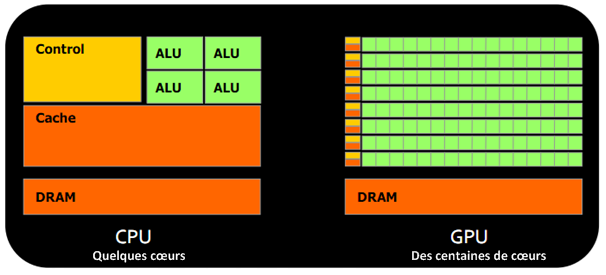
\includegraphics[width=0.8\textwidth]{im/archi-GPU-vs-CPU}
	\caption[Diferencia de arquitecturas entre CPU y GPU]{Diferencia de arquitecturas entre CPU y GPU\footnotemark}
	\label{fig:cvsg}
\end{figure}
\footnotetext{Imagen tomada de \url{http://imagefriend.com/cpu-vs-gpu.shtm}}

Al programar en el lenguaje nativo para las GPU's de NVIDIA, CUDA, se utilizan los cores de la GPU llamando threads dentro de la ejecución del programa. Cada thread es ejecutado en uno de los cores en un arreglo llamado bloque, el cual se ejecuta en un multiprocesador. Este concepto es importante debido a que por más que por más hilos o bloques que se llamen, sólo se ejecutarán a la vez los disponibles por hardware en la GPU, la cuál viene con una cantidad de multiprocesadores fija, cada uno con sus propios recursos, como se muestra en la Figura \ref{fig:multi}. Cada procesador escalar cuenta con su propio set de registros y todos tiene acceso a las memorias globales, bien sea la de la GPU, la constante o la de texturas. Pero de todas maneras cada uno de los multiprocesadores (o arreglo en bloque de procesadores escalares) cuenta con su propia memoria compartida. De manera que la manera en que se resuelve un problema no depende únicamente del problema en sí, sino que también de los recursos que se tengan disponibles para su programación. 

\begin{figure}[ht]
\centering
	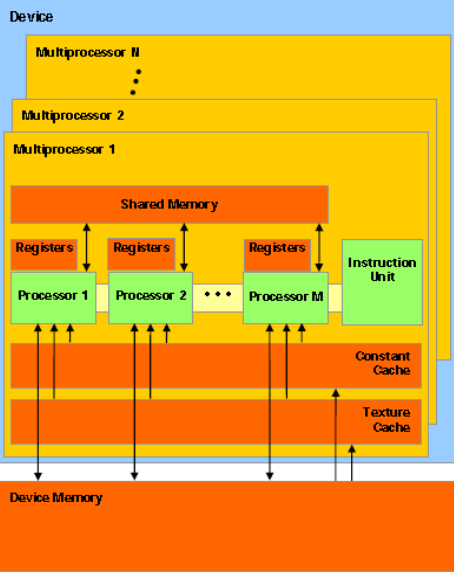
\includegraphics[width=0.55\textwidth]{im/arqui}
	\caption{Diferencia de arquitecturas entre CPU y GPU \cite{jpeg}}
	\label{fig:multi}
\end{figure}

Es importante tener en cuenta que el GPU no toma el control de las operaciones en general, sino que sigue bajo el mando del CPU. De manera que este último es el encargado de lanzar las funciones conocidas como kernels, las cuales se ejecutan en la GPU, especificando el arreglo de procesadores (hilos) que se van a utilizar y la geometría que van a ser, ya sea unidimensional o multidimensional, y de la misma manera la cantidad de bloques que se van a ejecutar en la GPU o grid.


\section{Justificación}
El ordenamiento de datos en forma de matrices es ampliamente usado en casi todos los ámbitos de la ciencia y tecnología, debido a que éste permite una mejor organización de los datos tanto como para fines prácticos como técnicos. Cualquier problema que se plantee en una situación multimensional o con una gran cantidad de datos o bien sea que utilicen álgebra lineal; bien sea problemas de optimización, física, química, entre otros, permitirán el uso de matrices. Si se requiere operar sobre dichas matrices o despejar algún grupo de términos lo más seguros es que inevitablemente se desemboque en una multiplicación de matrices. Dependiendo de la cantidad de datos o grados de libertad, estos problemas pueden crecer en gran medida y se vuelve necesario optimizar dicha multiplicación. Es por esto que este proyecto pretende introducir tanto el manejo de programación paralela de GPU mediante CUDA, así como diferentes aproximaciones que se pueden tener al manejar matrices, y mostrar las diferencias en tiempo de cada uno.

\section{Objetivos}
\begin{itemize}
	\item Encontrar diferentes mejoras ante diferentes algoritmos paralelos de multiplicación de matrices respecto al método secuencial
	\item Utilizar la memoria compartida y observar mejoras en los tiempos
	\item Generar una serie de códigos que se ejecuten en una GPU y sean funcionales para el propósito establecido
\end{itemize}
\newpage
\section{Desarrollo}
El desarrollo fue realizado en una Laptop Samsung que posee un procesador Intel de dos cores de segunda generación, y además una tarjeta gráfica NVIDIA GeForce 540M, que permitía un total de 1024 hilos por bloque, con dos multiprocesadores y 48kb de memoria compartida por cada uno. Fue muy importante tener estos aspectos en cuenta para el desarrollo del proyecto debido a que no sólo permitieron una correcta optimización y ejecución del programa, sino que también facilitaron encontrar errores y fallas.

\subsection{Multiplicación de Matrices: Secuencial}
Para realizar la multiplicación de matrices se debe explotar al máximo la capacidad de distribución de tareas de manera matricial dentro de la GPU, pero también se debe tener en cuenta que al transferir los datos del \textit{host} al \textit{device} se cuenta espacio limitado. Es importante también tomar en cuenta que la forma en que organicemos nuestros datos definirá lo rápido que se accede a memoria influyendo en el tiempo final de ejecución. 

Para el caso secuencial se siguió el código mostrado a continuación. Si bien dada la notación utilizada en el método escrito hace que sea mucho más sencillo crear arreglos bidimensionales, estos entorpecen el proceso y vuelven más lento el acceso a memoria, transformando las matrices a vectores, bien sea por columnas o por filas, es la mejor manera de trabajar con ellas.


\lstinputlisting[language=C, firstline=5, lastline=18]{../Mat_sec.c}

Aquí se realiza una doble iteración para recorrer la matriz resultado para la cual se realiza una última iteración para recorrer las filas de la primera matriz y las columnas de la segunda.

\subsection{Multiplicación de Matrices: Paralelo}
Para la multiplicación en paralelo se implementaron tres métodos más una implementación utilizando la memoria compartida. Los dos primeros métodos utilizan la misma metodología del algoritmo secuencial, salvo que sólo se ejecuta la última iteración debido a que organizando los \textit{threads} de manera matricial podemos ahorrarnos las dos primeras iteraciones. Para el primer algoritmo se realiza primero un cálculo bajo el cual se decide la cantidad de bloques e hilos (manteniendo al mínimo la cantidad de bloques ya que los multiprocesadores son recursos más limitados), teniendo en cuenta que el número de hilos por bloque no supere el límite establecido. Después de ello ejecuta el kernel (mostrado a continuación) y recupera los resultados.

\lstinputlisting[language=C, firstline=5, lastline=18]{../Mat_1.cu}

Para el segundo esquema de ejecución, se utiliza la idea de ejecutar todas las tareas en un único bloque, por lo cual se limitan los posibles tamaños de las matrices, pero como se mostrará en la Sección \ref{sec:res}, se muestra una mejoría considerable en el rendimiento.

Finalmente, para el tercer caso se optó por dividir las matrices entrantes en 4 partes iguales (creando la restricción de que sean matrices cuadradas de dimensión par) y multiplicando las partes correspondientes. Esto evita realizar recorridos largos, agregando más procesos por cada matriz, pero sobretodo puede evitar la necesidad de asignar grandes espacios de memoria en la GPU, debido a que se puede se puede ejecutar una sub-multiplicación a la vez. La idea general se muestra a continuación, 

\[ \begin{pmatrix} A_{UL}&A_{UR}\\A_{LL}&A_{LR}\end{pmatrix}\cdot\begin{pmatrix} B_{UL}&B_{UR}\\B_{LL}&B_{LR}\end{pmatrix}= \begin{pmatrix} C_{UL}&C_{UR}\\C_{LL}&C_{LR}\end{pmatrix} \]

\[ C=\begin{pmatrix} A_{UL}B_{UL}+A_{UR}B_{LL}& A_{UL}B_{UR}+A_{UR}B_{LR} \\A_{LL}B_{UL}+A_{LR}B_{LL}&A_{LL}B_{UR}+A_{LR}B_{LR}\end{pmatrix}  \]

Hay varias formas de realizar este algoritmo, entre ellas puede que la más efectiva sea lanzar 8 veces el kernel, realizando los preparativos correspondientes cada vez. Para este proyecto se optó por la que ofrecía una menor carga para la CPU, lo cual se hizo por el hecho de que es un ejemplo demostrativo, por lo cual no se van a realizar grandes multiplicaciones y habrá memoria suficiente en el GPU para albergar todas las submatrices a la vez. Como se ve en el código a continuación, una única ejecución del kernel realiza las 8 multiplicaciones. En caso contrario y la implementación demande altas prestaciones se debe extraer una a una las submatrices de la matriz principal e irlas enviando a la GPU para realizar la multiplicación. 
%\newpage
\lstinputlisting[language=C, firstline=5, lastline=40]{../Mat_3.cu}

Finalmente para la memoria compartida se fijó un tamaño de 31 para todas las ejecuciones (excepto para el tercer caso) para que el caso 2 pudiese operar en un único bloque sin desbordar el número de threads. Como se muestra a continuación, al entrar al kernel se copian las matrices a la memoria compartida y a partir de ellas se realiza el cálculo de la multiplicación.

\lstinputlisting[language=C, firstline=5, lastline=23]{../Mat_1_COMP.cu}

\newpage
\section{Resultados}
\label{sec:res}

Para obtener los resultados hubo varios problemas en cuestión de transferencia y uso de memoria, puesto que la cantidad de datos crece de manera cuadrática con respecto a la dimensión de la matriz. Es por esto que se tuvieron que agregar condiciones en busca de errores tanto al asignar la memoria en la GPU como en la copia de memoria hacia ésta. Además hubo problemas que se saltaron las comprobaciones sin haber respuesta aparente del programa, arrojando tiempos casi coherentes, los cuales sólo pudieron ser detectados imprimiendo regiones conocidas de la matriz de resultado. Por dichos problemas de memoria se tomaron los tiempos para los tamaños de 100, 200 y 500 (sólo el último método permitió una correcta multiplicación para matrices de 1000 x 1000). En la Tabla \ref{tab:tiempos} se muestran los tiempos obtenidos por multiplicación para cada una de las metodologías. 

\begin{table}[H]
\centering
	\begin{tabular}{rrrrrc}
		\hline\hline
		\textbf{Tamaño} & \textbf{Secuencial} & \textbf{Par 1} & \textbf{Par 2} & \textbf{Par 3}&\textbf{Compartida}\\
		\hline
		100 & 4.09 ms&0.201ms & 0.218 ms&0.105 ms&--\\
		200 &38.28 ms&2.12 ms &	0.182 ms	 & 0.78ms&--\\
		500	&979.22 ms&32.28 ms	&3.52 ms	&10.6 ms&--\\
		31 &--&14.3 us&14.9 us&11.6 us\footnotemark &6.38 us\\


		\hline
	\end{tabular}
	\caption{Tabla de tiempos}
	\label{tab:tiempos}
\end{table}
\footnotetext{Para el caso de la técnica de división de matrices se utilizó un tamaño de 32}

Es importante tener en cuenta que no todos los problemas (por sus algoritmos internos) utilizaron la misma distribución de bloques e hilos, la cual se puede observar en la Tabla \ref{tab:hilos}, teniendo en cuenta que para la técnica 3 estos bloques e hilos son por cada submatriz ingresada en el kernel. 

\begin{table}[H]
\centering
	\begin{tabular}{rrrrc}
		\hline\hline
		\textbf{Tamaño} & \textbf{Par 1} & \textbf{Par 2} & \textbf{Par 3}&\textbf{Compartida}\\
		\hline
		100 &  4x25 & 4x25&2x25&--\\
		200 & 7x29 &	7x29 & 4x25&--\\
		500	&16x32&16x32&16x16&--\\
		31 &1x31&1x31&1x16&1x31\\


		\hline
	\end{tabular}
	\caption{Tamaños de los kernels (bloquesxhilos)}
	\label{tab:hilos}
\end{table}

\section{Conclusiones}
Como se puede observar en la Tabla \ref{tab:tiempos} hay una mejoría considerable a la hora de realizar una multiplicación de matrices, debido a que se reduce de manera significativa el tiempo de ejecución. Realizando el cociente de los tiempos, notamos que para un tamaño de 100x100 la mejoría oscila entre 18.7 veces (Par 2) hasta 40 veces (Par 3). Por otro lado, para el caso de 500x500 la mejoría es de 30.33 veces para Par 1, 92.37 veces para Par 3, pero para el algoritmo Par 2 el speed-up es de un factor de 278.18 veces. Finalmente observamos que al utilizar la memoria compartida, la velocidad de ejecución tiende a duplicarse respecto al algoritmo base, que en este caso sería el Par 1.

Para trabajos futuros, queda realizar una optimización del uso de memoria, así como intentar con funciones como la cudaMemcpy2D que permite la manipulación de matrices. Para el caso del algoritmo Par 3 se recomienda intentar lanzar el kernel 8 veces con cada multiplicación mostrada anteriormente. De esta manera sólo se reserva la memoria correspondiente a 3 submatrices en la GPU, mientras que en la GPU sólo almacena las dos que se van a multiplicar en cada paso, a pesar de que se tienen que almacenar las 8 de salida. 
\nocite{*}
\bibliographystyle{apalike} 
\bibliography{references}
\end{document}	